\documentclass[12pt, oneside]{article}
\usepackage[letterpaper, margin=1in, headsep=0.5in]{geometry}
\usepackage[english]{babel}
\usepackage[utf8]{inputenc}
\usepackage{amsmath}
\usepackage{amsfonts}
\usepackage{amssymb}
\usepackage{tikz}
\usetikzlibrary{quotes, angles}
\usepackage{graphicx}
%\usepackage{pgfplots}
%\pgfplotsset{width=10cm,compat=1.9}
%\usepgfplotslibrary{statistics}
%\usepackage{pgfplotstable}
%\usepackage{tkz-fct}
%\usepackage{venndiagram}

\usepackage{fancyhdr}
\pagestyle{fancy}
\fancyhf{}
\rhead{\thepage \\Name: \hspace{1.5in}.\\}
\lhead{BECA / Dr. Huson / Geometry 10th Grade\\* Unit 1: Introduction to Geometry}

\renewcommand{\headrulewidth}{0pt}

\begin{document}
\subsubsection*{1-8 Homework: Pretest problems}
  \vspace{0.5cm}
  \begin{enumerate}
    \item Points that are all located on the same line are $\rule{4cm}{0.15mm}$.\bigskip


    \item Use symbols to write the name of each geometric figure.
    \begin{enumerate}
    \item %Ray DE
      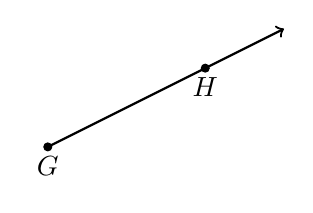
\begin{tikzpicture}
        \draw [->, thick] (0,0)--(3,1.5);
        \draw [fill] (0,0) circle [radius=0.05] node[below]{$G$};
        \draw [fill] (2,1) circle [radius=0.05] node[below]{$H$};
      \end{tikzpicture} \bigskip
    \item \hspace{1cm}%Line AB
      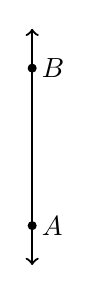
\begin{tikzpicture}
        \draw [<->, thick] (1,0)--(1,3);
        \draw [fill] (1,0.5) circle [radius=0.05] node[right]{$A$};
        \draw [fill] (1,2.5) circle [radius=0.05] node[right]{$B$};
      \end{tikzpicture} \bigskip
      \item %Line segment XY
        \begin{tikzpicture}
          \draw [-, thick] (1,0)--(0,2);
          \draw [fill] (1,0) circle [radius=0.05] node[below]{$E$};
          \draw [fill] (0,2) circle [radius=0.05] node[left]{$F$};
        \end{tikzpicture}
    \end{enumerate}

    \item A flat surface is a(n) $\rule{4cm}{0.15mm}$. \bigskip

    \item Find the value of $|2.5-3|$.

    \item Two line segments or angles of equal measure are $\rule{4cm}{0.15mm}$.
      \bigskip

    \item Given $\overline{ABC}$, $AB=3 \frac{1}{3}$, and $BC=1$.
    \begin{enumerate}
      \item Find ${AC}$.\\[0.75cm]
        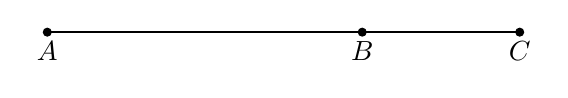
\begin{tikzpicture}
          \draw [-, thick] (1,0)--(7,0);
          \draw [fill] (1,0) circle [radius=0.05] node[below]{$A$};
          \draw [fill] (5,0) circle [radius=0.05] node[below]{$B$};
          \draw [fill] (7,0) circle [radius=0.05] node[below]{$C$};
        \end{tikzpicture} \bigskip
      \item The postulate used in this problem is the \rule{6cm}{0.15mm}.
    \end{enumerate}

    \newpage

    \item Identify two rays in the given plane.\\[0.25in]
      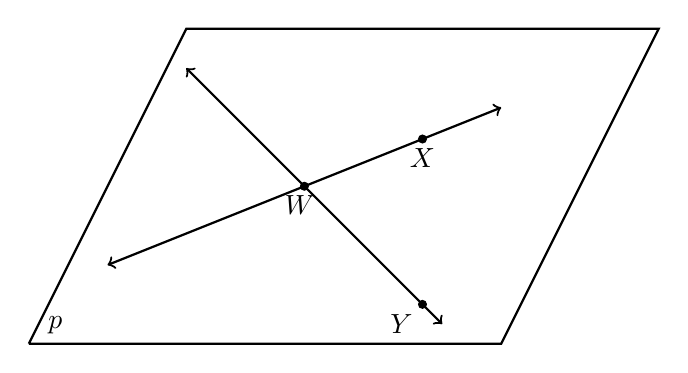
\begin{tikzpicture}
        \draw [thick](0,0) node[above right]{$\ p$} --(6,0)--(8,4)--(2,4)--(0,0);
        \draw [<->, thick] (1,1)--(6,3);
        \draw [fill] (3.5,2) circle [radius=0.05] node[below]{$W \ $};
        \draw [fill] (5,2.6) circle [radius=0.05] node[below]{$X$};
        \draw [<->, thick] (2,3.5)--(5.25,.25);
        \draw [fill] (5,0.5) circle [radius=0.05] node[below left]{$Y$};
      \end{tikzpicture} %\vspace{2cm}


      \item Use symbols to write the name of the given figure.
        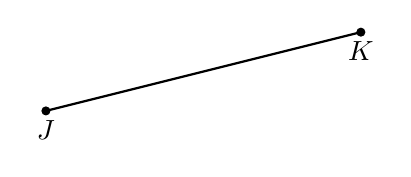
\begin{tikzpicture}
          \draw [-, thick] (0,0)--(4,1);
          \draw [fill] (0,0) circle [radius=0.05] node[below]{$J$};
          \draw [fill] (4,1) circle [radius=0.05] node[below]{$K$};
        \end{tikzpicture} \bigskip

      \item Draw and label a line segment $\overline AB$ such that the distance between points $A$ and $B$ is 6 cm. \vspace{2cm}


      \item Given $T(3,2)$ and $U(4,8)$. What is the slope of $\overleftrightarrow{TU}$? Use the formula $\displaystyle m=\frac{y_U-y_T}{x_U-x_T}$. \vspace{3cm}

      \item A(n) $\rule{4cm}{0.15mm}$ is a portion of a line that includes two points and all of the collinear points between the two points.\smallskip

      \newpage

      \item Given $\overline{ABC}$, $AB=2x-10$, $BC=x+2$, $AC=10$. Find ${BC}$.
      \begin{enumerate}
        \item Sketch and label the situation
        \begin{flushright}
          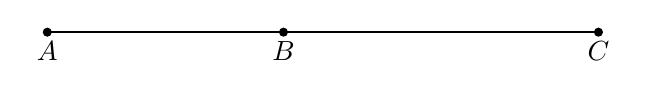
\begin{tikzpicture}
             \draw [-, thick] (0,0)--(7,0);
             \draw [fill] (0,0) circle [radius=0.05] node[below]{$A$};
             \draw [fill] (3,0) circle [radius=0.05] node[below]{$B$};
             \draw [fill] (7,0) circle [radius=0.05] node[below]{$C$};
          \end{tikzpicture}
        \end{flushright} \vspace{2cm}
        \item Write a geometric equation: \rule{5cm}{0.15mm} \vspace{1cm}
        \item Substitute algebraic values: \rule{5cm}{0.15mm}
        \item Solve for $x$
        \vspace{4cm}
        \begin{center} $x=$ \rule{1cm}{0.15mm} \end{center}
        \item Answer the question: Find $BC$ by substituting for $x$. \bigskip
        \begin{center} $BC=($ \hspace{1cm} $)+2=$ \rule{1cm}{0.15mm} \end{center} \bigskip
        \item Check your answer
      \end{enumerate}
      \vspace{2cm}

      \newpage
      \item Given $m\angle LKM = 5x+10$, $m\angle MKN = 3x+5$, and $m\angle LKN = 130$, find $m\angle MKN$.  \vspace{.2cm}
      \begin{enumerate}
        \item Sketch and label the situation
        \begin{flushright}
        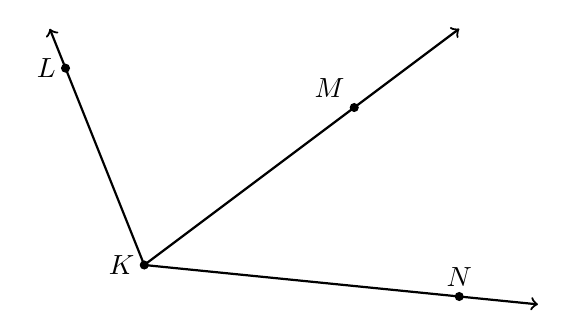
\begin{tikzpicture}[scale=1]
          \draw [->, thick] (0,0)--(4,3);
          \draw [->, thick] (0,0)--(5,-.5);
          \draw [->, thick] (0,0)--(-1.2,3);
          \draw [fill] (-1,2.5) circle [radius=0.05] node[left ]{$L$};
          \draw [fill] (2.66666,2) circle [radius=0.05] node[above left ]{$M$};
          \draw [fill] (0,0) circle [radius=0.05] node[left]{$K$};
          \draw [fill] (4,-0.4) circle [radius=0.05] node[above]{$N$};
        \end{tikzpicture}
        \end{flushright}
        \vspace{1cm}

        \item Write a geometric equation: \rule{5cm}{0.15mm} \vspace{1cm}
        \item Substitute algebraic values: \rule{5cm}{0.15mm}
        \item Solve for $x$
        \vspace{4cm}
        \begin{center} $x=$ \rule{1cm}{0.15mm} \end{center}
        \item Answer the question: Find $m\angle MKN$ by substituting for $x$.  \bigskip
        \begin{center} $m\angle MKN=3($ \hspace{1cm} $)+5=$ \rule{1cm}{0.15mm} \end{center}
        \item Check your answer
      \end{enumerate}
      \vspace{2cm}
    \end{enumerate}

\newpage
\setcounter{page}{1}
  \subsubsection*{Exam: Tools of Geometry}
    \vspace{0.5cm}
    \begin{enumerate}
      \item Points that are all located on the same plane are $\rule{4cm}{0.15mm}$.\bigskip


      \item Draw and label a line segment $\overline{AB}$ such that the distance between points $A$ and $B$ is 4 cm. \vspace{2cm}


      \item Identify three points in the given plane.\\[0.25in]
        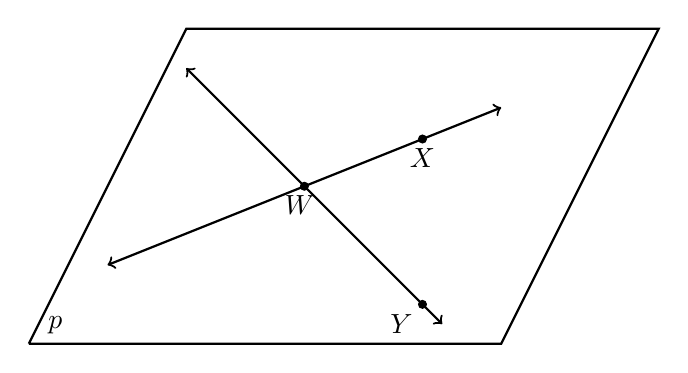
\begin{tikzpicture}
          \draw [thick](0,0) node[above right]{$\ p$} --(6,0)--(8,4)--(2,4)--(0,0);
          \draw [<->, thick] (1,1)--(6,3);
          \draw [fill] (3.5,2) circle [radius=0.05] node[below]{$W \ $};
          \draw [fill] (5,2.6) circle [radius=0.05] node[below]{$X$};
          \draw [<->, thick] (2,3.5)--(5.25,.25);
          \draw [fill] (5,0.5) circle [radius=0.05] node[below left]{$Y$};
        \end{tikzpicture} \vspace{1cm}


      \item A flat surface is a(n) $\rule{4cm}{0.15mm}$. \bigskip

      \item Find the value of $|5-3|+|4-5|$. \bigskip

      \item Two line segments or angles of equal measure are $\rule{4cm}{0.15mm}$.
        \bigskip

      \item Given $\overline{DEF}$, $DE=5 \frac{1}{2}$, and $EF=2 \frac{1}{2}$.
      \begin{enumerate}
        \item Find ${DF}$.\\[.5in]
          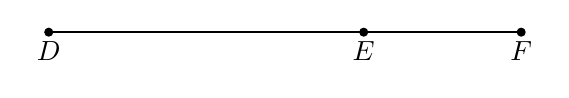
\begin{tikzpicture}
            \draw [-, thick] (1,0)--(7,0);
            \draw [fill] (1,0) circle [radius=0.05] node[below]{$D$};
            \draw [fill] (5,0) circle [radius=0.05] node[below]{$E$};
            \draw [fill] (7,0) circle [radius=0.05] node[below]{$F$};
          \end{tikzpicture} \bigskip
        \item The postulate used in this problem is the \rule{6cm}{0.15mm}.
      \end{enumerate}

      \newpage
      \item Given the points $V$ and $W$, draw $\overrightarrow{WV}$.\\
      \vspace{1cm}
      \begin{center}
        \begin{tikzpicture}
        \draw [fill] (0,2) circle [radius=0.05] node[below]{$V$};
        \draw [fill] (5,0) circle [radius=0.05] node[below]{$W$};
      \end{tikzpicture}
      \end{center}
      \vspace{1cm}

      \item Use symbols to write the name of each geometric figure.\\.\\
      \vspace{0.5cm}
      \begin{tikzpicture}
        \draw [->, thick] (0,0)--(3,1.5);
        \draw [fill] (0,0) circle [radius=0.05] node[below]{$G$};
        \draw [fill] (2,1) circle [radius=0.05] node[below]{$H$};
        \node at (-1,0) {(a)};
      \end{tikzpicture}  \hspace{.1cm}
      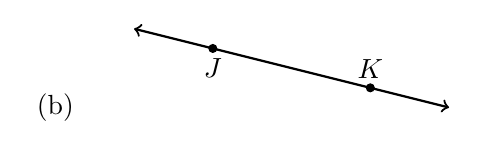
\begin{tikzpicture}
        \draw [<->, thick] (1,1)--(5,0);
        \draw [fill] (2,0.75) circle [radius=0.05] node[below]{$J$};
        \draw [fill] (4,.25) circle [radius=0.05] node[above]{$K$};
        \node at (0,0) {(b)};
      \end{tikzpicture} \hspace{.25cm}
      \begin{tikzpicture}
        \draw [-, thick] (1,0)--(4,2);
        \draw [fill] (1,0) circle [radius=0.05] node[below]{$L$};
        \draw [fill] (4,2) circle [radius=0.05] node[above left]{$M$};
        \node at (0,0) {(c)};
      \end{tikzpicture}
      \vspace{1cm}

      \item Given $P(6,5)$ and $Q(4,7)$. What is the slope of $\overleftrightarrow{PQ}$? Use the formula $\displaystyle m=\frac{y_Q-y_P}{x_Q-x_P}$. \vspace{3cm}

      \item Using a straightedge, draw a pair of opposite rays. Label any points in the drawing and name the two rays to the right of the drawing, using proper notation.\smallskip

      \newpage
      \item Given $\triangle JKL$ with $\overline{JK} \cong \overline{KL}$. On the diagram mark the congruent line segments with tick marks.
      \begin{center}
      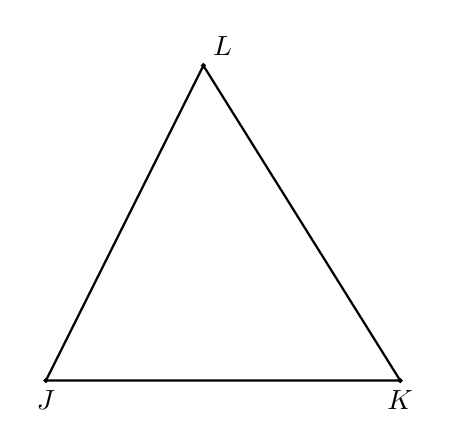
\begin{tikzpicture}[scale=0.5]
        \draw [thick](0,0)--(9,0)--(4,8)--(0,0);
        \draw [fill] (0,0) circle [radius=0.05] node[below]{$J$};
        \draw [fill] (9,0) circle [radius=0.05] node[below]{$K$};
        \draw [fill] (4,8) circle [radius=0.05] node[above right]{$L$};
      \end{tikzpicture}
      \end{center}
      \vspace{1cm}


      \item Find the measure of the angle in degrees and the given segment's length in centimeters. \vspace{0.25cm}
      \begin{enumerate}
        \item  $m \angle UST = $ \rule{4cm}{0.15mm} \bigskip
        \item  $SU=$ \rule{4cm}{0.15mm} \bigskip
        \item Name a pair of opposite rays: \rule{4cm}{0.15mm} \bigskip
      \end{enumerate}
      \begin{center}
      \begin{tikzpicture}[scale=1.5]
        \draw [->, thick] (0,0)--(4,4);
        \draw [<->, thick] (-3,0)--(7,0);
        %\draw [->, thick] (0,0)--(-1.2,3);
        %\draw [fill] (-1,2.5) circle [radius=0.05] node[left ]{$B$};
        \draw [fill] (3,3) circle [radius=0.05] node[above left ]{$U$};
        \draw [fill] (-2,0) circle [radius=0.05] node[below]{$R$};
        \draw [fill] (0,0) circle [radius=0.05] node[below]{$S$};
        \draw [fill] (4,0) circle [radius=0.05] node[above]{$T$};
      \end{tikzpicture}
      \end{center}

  \newpage

        \item Given $\overline{ABC}$, $AB=3x-4$, $BC=x+5$, $AC=13$. Find ${BC}$.
        \begin{enumerate}
          \item Sketch and label the situation
          \begin{flushright}
            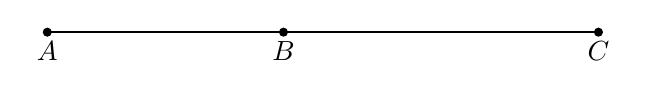
\begin{tikzpicture}
               \draw [-, thick] (0,0)--(7,0);
               \draw [fill] (0,0) circle [radius=0.05] node[below]{$A$};
               \draw [fill] (3,0) circle [radius=0.05] node[below]{$B$};
               \draw [fill] (7,0) circle [radius=0.05] node[below]{$C$};
            \end{tikzpicture}
          \end{flushright} \vspace{2cm}
          \item Write a geometric equation: \rule{5cm}{0.15mm} \vspace{1.5cm}
          \item Substitute algebraic values: \rule{5cm}{0.15mm} \bigskip
          \item Solve for $x$
          \vspace{5cm}
          \begin{center} $x=$ \rule{1cm}{0.15mm} \end{center} \bigskip
          \item Answer the question: Find $BC$ by substituting for $x$. \bigskip
          \begin{center} $BC=($ \hspace{1cm} $)+5=$ \rule{1cm}{0.15mm} \end{center} \bigskip
          \item Check your answer
        \end{enumerate}
        \vspace{2cm}

  \newpage
        \item Given $\angle ADB$ with angle bisector $\overrightarrow{DC}$. $m\angle ADC = 4x+2$, $m\angle BDC = 3x+14$. Find $m\angle ADC$.  %\vspace{.2cm}
        \begin{enumerate}
          \item Sketch and label the situation
          \begin{flushright}
          \begin{tikzpicture}[scale=1]
            \draw [->, thick] (0,0)--(3.5,4.375);
            \draw [->, thick] (0,0)--(5,0);
            \draw [->, thick] (0,0)--(-1.8,4.5);
            \draw [fill] (-1,2.5) circle [radius=0.05] node[left ]{$A$};
            \draw [fill] (3,3.75) circle [radius=0.05] node[above left ]{$C$};
            \draw [fill] (0,0) circle [radius=0.05] node[left]{$D$};
            \draw [fill] (4,0) circle [radius=0.05] node[above]{$B$};
          \end{tikzpicture}
          \end{flushright}
          \vspace{.5cm}

          \item Write a geometric equation: \rule{5cm}{0.15mm} \vspace{1cm}
          \item Substitute algebraic values: \rule{5cm}{0.15mm}
          \item Solve for $x$
          \vspace{4cm}
          \begin{center} $x=$ \rule{1cm}{0.15mm} \end{center}
          \item Answer the question: Find $m\angle ADC$ by substituting for $x$. \vspace{2cm}
          \begin{center} $m\angle ADC=$ \rule{1cm}{0.15mm} \end{center}
          \item Check your answer
        \end{enumerate}
        \vspace{2cm}

        \newpage
        \item Complete the construction of an equilateral triangle including the six steps.
        \begin{enumerate}
          \item Given the line segment $\overline{MN}$.
          \bigskip
          \item Construct circle $M$ with radius $\rule{2cm}{0.15mm}$.
          \bigskip
          \item Construct circle $\rule{2cm}{0.15mm}$  with radius $\rule{2cm}{0.15mm}$. \bigskip
          \item Label the intersection $P$ of the two circles.
          \bigskip
          \item Draw line segments $\rule{2cm}{0.15mm}$  and $\rule{2cm}{0.15mm}$
          \bigskip
          \item $\triangle MNP$ is equilateral.
        \end{enumerate}
        \vspace{7cm}
        \begin{center}
        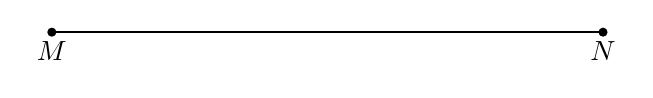
\begin{tikzpicture}
          \draw [-, thick] (0,0)--(7,0);
          \draw [fill] (0,0) circle [radius=0.05] node[below]{$M$};
          \draw [fill] (7,0) circle [radius=0.05] node[below]{$N$};
        \end{tikzpicture}
        \end{center}

    \end{enumerate}

    \newpage
    \setcounter{page}{5}
      \emph{Spicy}\\
      15b. Given $\angle ADB$ with angle bisector $\overrightarrow{DC}$ and $m\angle ADC = 4x+2$, $m\angle ADB = 7x+16$. Find $m\angle BDC$.  %\vspace{.2cm}
      \begin{enumerate}
        \item Sketch and label the situation
        \begin{flushright}
        \begin{tikzpicture}[scale=1]
          \draw [->, thick] (0,0)--(3.5,4.375);
          \draw [->, thick] (0,0)--(5,0);
          \draw [->, thick] (0,0)--(-1.8,4.5);
          \draw [fill] (-1,2.5) circle [radius=0.05] node[left ]{$A$};
          \draw [fill] (3,3.75) circle [radius=0.05] node[above left ]{$C$};
          \draw [fill] (0,0) circle [radius=0.05] node[left]{$D$};
          \draw [fill] (4,0) circle [radius=0.05] node[above]{$B$};
        \end{tikzpicture}
        \end{flushright}
        \vspace{.5cm}

        \item Write a geometric equation: \rule{5cm}{0.15mm} \vspace{1cm}
        \item Substitute algebraic values: \rule{5cm}{0.15mm}
        \item Solve for $x$
        \vspace{4cm}
        \begin{center} $x=$ \rule{1cm}{0.15mm} \end{center}
        \item Answer the question: Find $m\angle BDC$ %by substituting for $x$.
        \vspace{2cm}
        \begin{center} $m\angle BDC=$ \rule{1cm}{0.15mm} \end{center}
        \item Check your answer
      \end{enumerate}
      \vspace{2cm}

      \newpage
      \emph{Spicy}\\
      16b. Complete the construction of an equilateral triangle including the six steps.
      \begin{enumerate}
        \item Given the line segment $\overline{MN}$.
        \bigskip
        \item %Construct circle $M$ with radius $\rule{2cm}{0.15mm}$.
        \bigskip
        \item %Construct circle $\rule{2cm}{0.15mm}$  with radius $\rule{2cm}{0.15mm}$.
        \bigskip
        \item %Label the intersection $P$ of the two circles.
        \bigskip
        \item %Draw line segments $\rule{2cm}{0.15mm}$  and $\rule{2cm}{0.15mm}$
        \bigskip
        \item $\triangle MNP$ is equilateral.
      \end{enumerate}
      \vspace{7cm}
      \begin{center}
      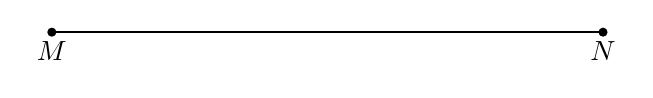
\begin{tikzpicture}
        \draw [-, thick] (0,0)--(7,0);
        \draw [fill] (0,0) circle [radius=0.05] node[below]{$M$};
        \draw [fill] (7,0) circle [radius=0.05] node[below]{$N$};
      \end{tikzpicture}
      \end{center}

\newpage
\setcounter{page}{1}
  \subsubsection*{Exam Corrections: Tools of Geometry}
  \emph{Study your errors. For each, write a note to yourself: what you need to do differently.\\ Do all problems in this handout.}
    \vspace{0.5cm}
    \begin{enumerate}
    \item Points that are all located on the same line are $\rule{4cm}{0.15mm}$.\bigskip


    \item Draw and label a line segment $\overline{AB}$ such that the distance between points $A$ and $B$ is 4 cm. \vspace{2cm}


    \item Identify three line segments in the given plane.\\[0.25in]
      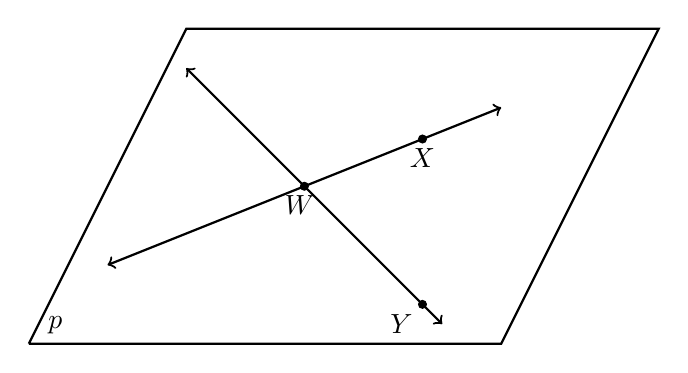
\begin{tikzpicture}
        \draw [thick](0,0) node[above right]{$\ p$} --(6,0)--(8,4)--(2,4)--(0,0);
        \draw [<->, thick] (1,1)--(6,3);
        \draw [fill] (3.5,2) circle [radius=0.05] node[below]{$W \ $};
        \draw [fill] (5,2.6) circle [radius=0.05] node[below]{$X$};
        \draw [<->, thick] (2,3.5)--(5.25,.25);
        \draw [fill] (5,0.5) circle [radius=0.05] node[below left]{$Y$};
      \end{tikzpicture} \vspace{1cm}


    \item A flat surface is a(n) $\rule{4cm}{0.15mm}$. \bigskip

    \item Find the value of $|15-3|+|4-15|$. \bigskip

    \item Two line segments or angles of equal measure are $\rule{4cm}{0.15mm}$.
      \bigskip

    \item Given $\overline{DEF}$, $DE=4 \frac{1}{5}$, and $EF=1 \frac{3}{5}$.
    \begin{enumerate}
      \item Find ${DF}$.\\[.5in]
        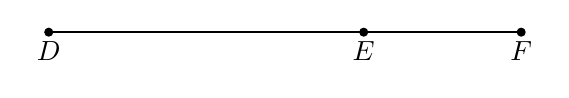
\begin{tikzpicture}
          \draw [-, thick] (1,0)--(7,0);
          \draw [fill] (1,0) circle [radius=0.05] node[below]{$D$};
          \draw [fill] (5,0) circle [radius=0.05] node[below]{$E$};
          \draw [fill] (7,0) circle [radius=0.05] node[below]{$F$};
        \end{tikzpicture} \bigskip
      \item The postulate used in this problem is the \rule{6cm}{0.15mm}.
    \end{enumerate}

    \newpage
    \item Given the points $V$ and $W$, draw $\overline{VW}$.\\
    \vspace{1cm}
    \begin{center}
      \begin{tikzpicture}
      \draw [fill] (0,2) circle [radius=0.05] node[below]{$V$};
      \draw [fill] (5,0) circle [radius=0.05] node[below]{$W$};
    \end{tikzpicture}
    \end{center}
    \vspace{1cm}

    \item Use symbols to write the name of each geometric figure.\\.\\
    \vspace{0.5cm}
    \begin{tikzpicture}
      \draw [-, thick] (1,0)--(4,2);
      \draw [fill] (1,0) circle [radius=0.05] node[below]{$L$};
      \draw [fill] (4,2) circle [radius=0.05] node[above left]{$M$};
      \node at (0,0) {(a)};
    \end{tikzpicture} \hspace{.1cm}
    \begin{tikzpicture}
      \draw [->, thick] (0,0)--(3,1.5);
      \draw [fill] (0,0) circle [radius=0.05] node[below]{$G$};
      \draw [fill] (2,1) circle [radius=0.05] node[below]{$H$};
      \node at (-1,0) {(b)};
    \end{tikzpicture}  \hspace{.1cm}
    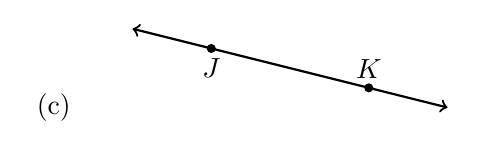
\begin{tikzpicture}
      \draw [<->, thick] (1,1)--(5,0);
      \draw [fill] (2,0.75) circle [radius=0.05] node[below]{$J$};
      \draw [fill] (4,.25) circle [radius=0.05] node[above]{$K$};
      \node at (0,0) {(c)};
    \end{tikzpicture}
    \vspace{1cm}

    \item Given $P(-2,5)$ and $Q(4,-7)$. What is the slope of $\overleftrightarrow{PQ}$? Use the formula $\displaystyle m=\frac{y_Q-y_P}{x_Q-x_P}$. \vspace{3cm}

    \item Using a straightedge, draw a pair of opposite rays. Label any points in the drawing and name the two rays to the right of the drawing, using proper notation.\smallskip

    \newpage
    \item Given $\triangle JKL$ with $\overline{JK} \cong \overline{JL}$. On the diagram mark the congruent line segments with tick marks.
    \begin{center}
    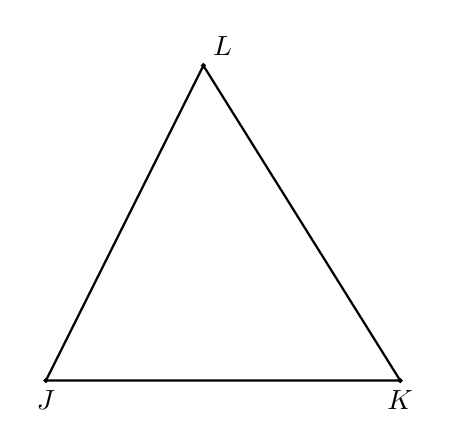
\begin{tikzpicture}[scale=0.5]
      \draw [thick](0,0)--(9,0)--(4,8)--(0,0);
      \draw [fill] (0,0) circle [radius=0.05] node[below]{$J$};
      \draw [fill] (9,0) circle [radius=0.05] node[below]{$K$};
      \draw [fill] (4,8) circle [radius=0.05] node[above right]{$L$};
    \end{tikzpicture}
    \end{center}
    \vspace{1cm}


    \item Find the measure of the angle in degrees and the given segment's length in centimeters. \vspace{0.25cm}
    \begin{enumerate}
      \item  $m \angle UST = $ \rule{4cm}{0.15mm} \bigskip
      \item  $SU=$ \rule{4cm}{0.15mm} \bigskip
      \item Name a pair of opposite rays: \rule{4cm}{0.15mm} \bigskip
    \end{enumerate}
    \begin{center}
    \begin{tikzpicture}[scale=1.5]
      \draw [->, thick] (0,0)--(3,4);
      \draw [<->, thick] (-3,0)--(7,0);
      %\draw [->, thick] (0,0)--(-1.2,3);
      %\draw [fill] (-1,2.5) circle [radius=0.05] node[left ]{$B$};
      \draw [fill] (2.25,3) circle [radius=0.05] node[above left ]{$U$};
      \draw [fill] (-2,0) circle [radius=0.05] node[below]{$R$};
      \draw [fill] (0,0) circle [radius=0.05] node[below]{$S$};
      \draw [fill] (4,0) circle [radius=0.05] node[above]{$T$};
    \end{tikzpicture}
    \end{center}

\newpage

      \item Given $\overline{ABC}$, $AB=3x-4$, $BC=x+5$, $AC=21$. Find ${BC}$.
      \begin{enumerate}
        \item Sketch and label the situation
        \begin{flushright}
          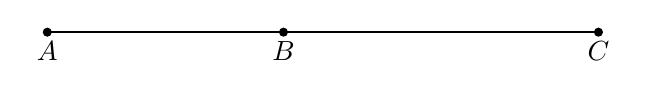
\begin{tikzpicture}
             \draw [-, thick] (0,0)--(7,0);
             \draw [fill] (0,0) circle [radius=0.05] node[below]{$A$};
             \draw [fill] (3,0) circle [radius=0.05] node[below]{$B$};
             \draw [fill] (7,0) circle [radius=0.05] node[below]{$C$};
          \end{tikzpicture}
        \end{flushright} \vspace{2cm}
        \item Write a geometric equation: \rule{5cm}{0.15mm} \vspace{1.5cm}
        \item Substitute algebraic values: \rule{5cm}{0.15mm} \bigskip
        \item Solve for $x$
        \vspace{5cm}
        \begin{center} $x=$ \rule{1cm}{0.15mm} \end{center} \bigskip
        \item Answer the question: Find $BC$ by substituting for $x$. \bigskip
        \begin{center} $BC=($ \hspace{1cm} $)+5=$ \rule{1cm}{0.15mm} \end{center} \bigskip
        \item Check your answer
      \end{enumerate}
      \vspace{2cm}

\newpage
      \item Given $\angle ADB$ with angle bisector $\overrightarrow{DC}$. $m\angle ADC = 5x-5$, $m\angle BDC = 3x+19$. Find $m\angle ADC$.  %\vspace{.2cm}
      \begin{enumerate}
        \item Sketch and label the situation
        \begin{flushright}
        \begin{tikzpicture}[scale=1]
          \draw [->, thick] (0,0)--(3.5,4.375);
          \draw [->, thick] (0,0)--(5,0);
          \draw [->, thick] (0,0)--(-1.8,4.5);
          \draw [fill] (-1,2.5) circle [radius=0.05] node[left ]{$A$};
          \draw [fill] (3,3.75) circle [radius=0.05] node[above left ]{$C$};
          \draw [fill] (0,0) circle [radius=0.05] node[left]{$D$};
          \draw [fill] (4,0) circle [radius=0.05] node[above]{$B$};
        \end{tikzpicture}
        \end{flushright}
        \vspace{.5cm}

        \item Write a geometric equation: \rule{5cm}{0.15mm} \vspace{1cm}
        \item Substitute algebraic values: \rule{5cm}{0.15mm}
        \item Solve for $x$
        \vspace{4cm}
        \begin{center} $x=$ \rule{1cm}{0.15mm} \end{center}
        \item Answer the question: Find $m\angle ADC$ by substituting for $x$. \vspace{2cm}
        \begin{center} $m\angle ADC=$ \rule{1cm}{0.15mm} \end{center}
        \item Check your answer
      \end{enumerate}
      \vspace{2cm}

      \newpage
      \item Complete the construction of an equilateral triangle including the six steps.
      \begin{enumerate}
        \item Given the line segment $\overline{MN}$.
        \bigskip
        \item Construct circle $M$ with radius $\rule{2cm}{0.15mm}$.
        \bigskip
        \item Construct circle $\rule{2cm}{0.15mm}$  with radius $\rule{2cm}{0.15mm}$. \bigskip
        \item Label the intersection $P$ of the two circles.
        \bigskip
        \item Draw line segments $\rule{2cm}{0.15mm}$  and $\rule{2cm}{0.15mm}$
        \bigskip
        \item $\triangle MNP$ is equilateral.
      \end{enumerate}
      \vspace{7cm}
      \begin{center}
      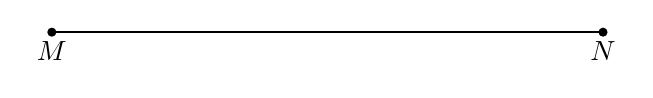
\begin{tikzpicture}
        \draw [-, thick] (0,0)--(7,0);
        \draw [fill] (0,0) circle [radius=0.05] node[below]{$M$};
        \draw [fill] (7,0) circle [radius=0.05] node[below]{$N$};
      \end{tikzpicture}
      \end{center}

  \end{enumerate}

  \newpage
  \setcounter{page}{5}
    \emph{Spicy}\\
    15b. Given $\angle ADB$ with angle bisector $\overrightarrow{DC}$ and $m\angle ADC = 5x-5$, $m\angle ADB = 8x+14$. Find $m\angle BDC$.  %\vspace{.2cm}
    \begin{enumerate}
      \item Sketch and label the situation
      \begin{flushright}
      \begin{tikzpicture}[scale=1]
        \draw [->, thick] (0,0)--(3.5,4.375);
        \draw [->, thick] (0,0)--(5,0);
        \draw [->, thick] (0,0)--(-1.8,4.5);
        \draw [fill] (-1,2.5) circle [radius=0.05] node[left ]{$A$};
        \draw [fill] (3,3.75) circle [radius=0.05] node[above left ]{$C$};
        \draw [fill] (0,0) circle [radius=0.05] node[left]{$D$};
        \draw [fill] (4,0) circle [radius=0.05] node[above]{$B$};
      \end{tikzpicture}
      \end{flushright}
      \vspace{.5cm}

      \item Write a geometric equation: \rule{5cm}{0.15mm} \vspace{1cm}
      \item Substitute algebraic values: \rule{5cm}{0.15mm}
      \item Solve for $x$
      \vspace{4cm}
      \begin{center} $x=$ \rule{1cm}{0.15mm} \end{center}
      \item Answer the question: Find $m\angle BDC$ %by substituting for $x$.
      \vspace{2cm}
      \begin{center} $m\angle BDC=$ \rule{1cm}{0.15mm} \end{center}
      \item Check your answer
    \end{enumerate}
    \vspace{2cm}

    \newpage
    \emph{Spicy}\\
    16b. Complete the construction of an equilateral triangle including the six steps.
    \begin{enumerate}
      \item Given the line segment $\overline{MN}$.
      \bigskip
      \item %Construct circle $M$ with radius $\rule{2cm}{0.15mm}$.
      \bigskip
      \item %Construct circle $\rule{2cm}{0.15mm}$  with radius $\rule{2cm}{0.15mm}$.
      \bigskip
      \item %Label the intersection $P$ of the two circles.
      \bigskip
      \item %Draw line segments $\rule{2cm}{0.15mm}$  and $\rule{2cm}{0.15mm}$
      \bigskip
      \item $\triangle MNP$ is equilateral.
    \end{enumerate}
    \vspace{7cm}
    \begin{center}
    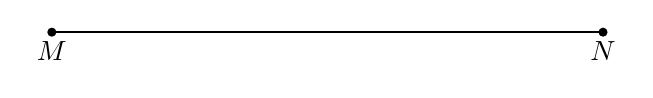
\begin{tikzpicture}
      \draw [-, thick] (0,0)--(7,0);
      \draw [fill] (0,0) circle [radius=0.05] node[below]{$M$};
      \draw [fill] (7,0) circle [radius=0.05] node[below]{$N$};
    \end{tikzpicture}
    \end{center}

\end{document}


      \item Spicy: Given the rectangle $ABCD$ with $\overline{AB} \cong \overline{CD}$ and $\overline{BC} \cong \overline{DA}$. $AB=x+7$ and $\displaystyle CD=\frac{4x+2}{2}$. Find $AB$.\\[0.5cm]
      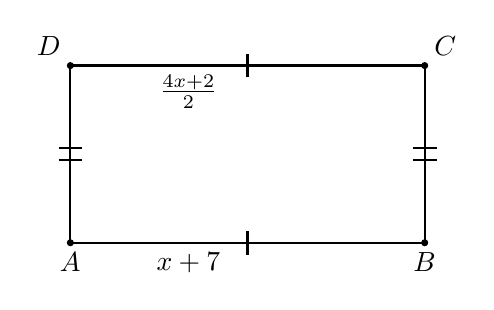
\begin{tikzpicture}[scale=0.75]
        \draw [thick](0,0)--(6,0)--(6,3)--(0,3)--(0,0);
        \draw [fill] (0,0) circle [radius=0.05] node[below]{$A$};
        \draw [fill] (6,0) circle [radius=0.05] node[below]{$B$};
        \draw [fill] (6,3) circle [radius=0.05] node[above right]{$C$};
        \draw [fill] (0,3) circle [radius=0.05] node[above left]{$D$};
        \draw [thick] (3,-0.2)--(3,0.2); %tick mark
        \draw [thick] (3,2.8)--(3,3.2); %tick mark
        \draw [thick] (-0.2,1.4)--(0.2,1.4); %tick mark
        \draw [thick] (-0.2,1.6)--(0.2,1.6); %tick mark
        \draw [thick] (5.8,1.4)--(6.2,1.4); %tick mark
        \draw [thick] (5.8,1.6)--(6.2,1.6); %tick mark
        \node [below] at (2,0){$x+7$};
        \node [below] at (2,3){$\frac{4x+2}{2}$};
      \end{tikzpicture}
      %\vspace{4cm}
